\documentclass[12pt]{article}
\usepackage[utf8]{inputenc}
\usepackage[T1]{fontenc}
\usepackage[french]{babel}
\usepackage{graphicx}
\usepackage{hyperref}
\usepackage{geometry}
\usepackage{float}

\geometry{a4paper, margin=1in}

\begin{document}

\begin{titlepage}
    \centering
    
\includegraphics[width=0.4\textwidth]{logo.png}\par\vspace{1cm}
    \vspace{2cm}
    {\huge\bfseries Compte Rendu IoT\par}
    \vspace{0.5cm}
    {\Large\bfseries TP 02: NodeRed, MQTT, NodeMCU\par}
    \vspace{2.5cm}
    {\large
    \begin{tabular}{rl}
      \textbf{Module:} & Internet des Objets (IoT) \\[0.8em]
      \textbf{Niveau:}  & IAGI - 2\textsuperscript{ème} année \\[0.8em]
      \textbf{Encadrant:} & Prof. Hain \\[0.8em]
      \textbf{Auteurs:} & Rabya RAGHIB \\
                        & Imane SAOUDI \\
                        & Nouhaila NOKRY \\
                        & Abdellah MOGHANDEZ \\
                        & Mohamed AMANE
    \end{tabular}}
    \vspace{2cm}
    
    \vfill
    {\large Année universitaire 2025/2026\par}
\end{titlepage}

\clearpage

\section*{Notre Équipe}

\begin{figure}[H]
    \centering
    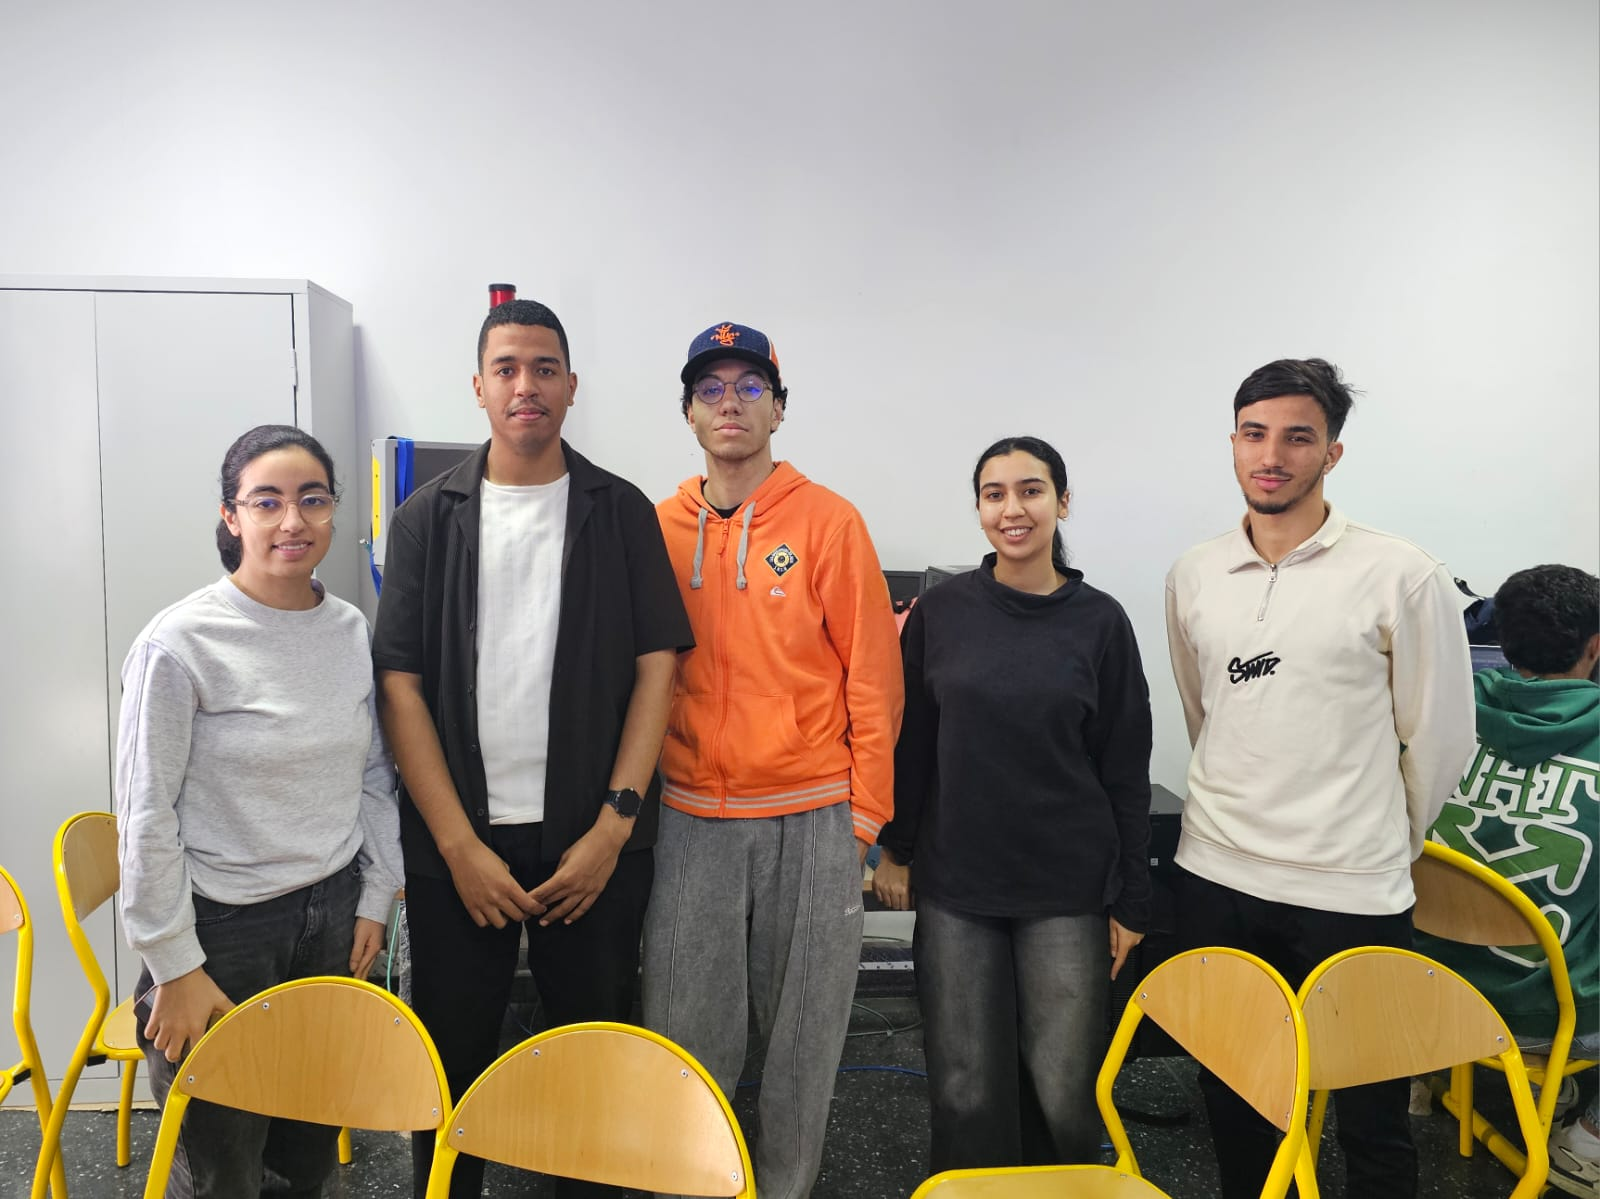
\includegraphics[width=0.8\textwidth]{team.jpeg}
    \caption{Photo de notre équipe}
\end{figure}

\clearpage

\section*{Atelier 15}

\textbf{Description :} Réalisation physique d'un montage permettant de contrôler à distance une LED connectée à un NodeMCU. En envoyant des messages (\texttt{on}, \texttt{off}) via le broker HiveMQ, le NodeMCU lit le topic et met à jour l'état de la LED.

\vspace{0.5cm}

\subsection*{Montage Circuit}

\begin{figure}[H]
    \centering
    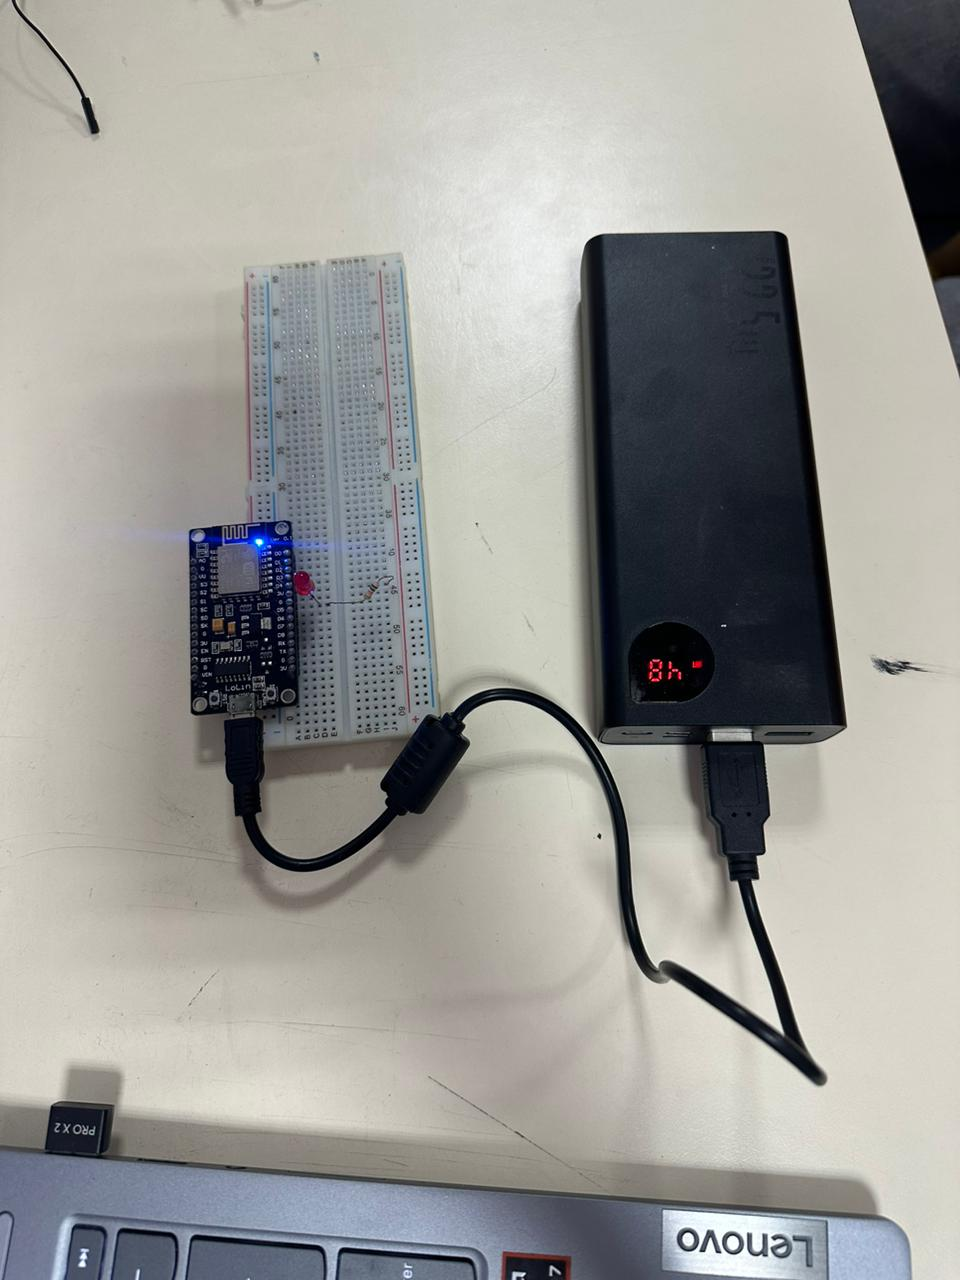
\includegraphics[width=0.6\textwidth]{../A15_Physical/circuit-off.jpeg}
    \caption{Circuit physique - LED éteinte}
\end{figure}

\begin{figure}[H]
    \centering
    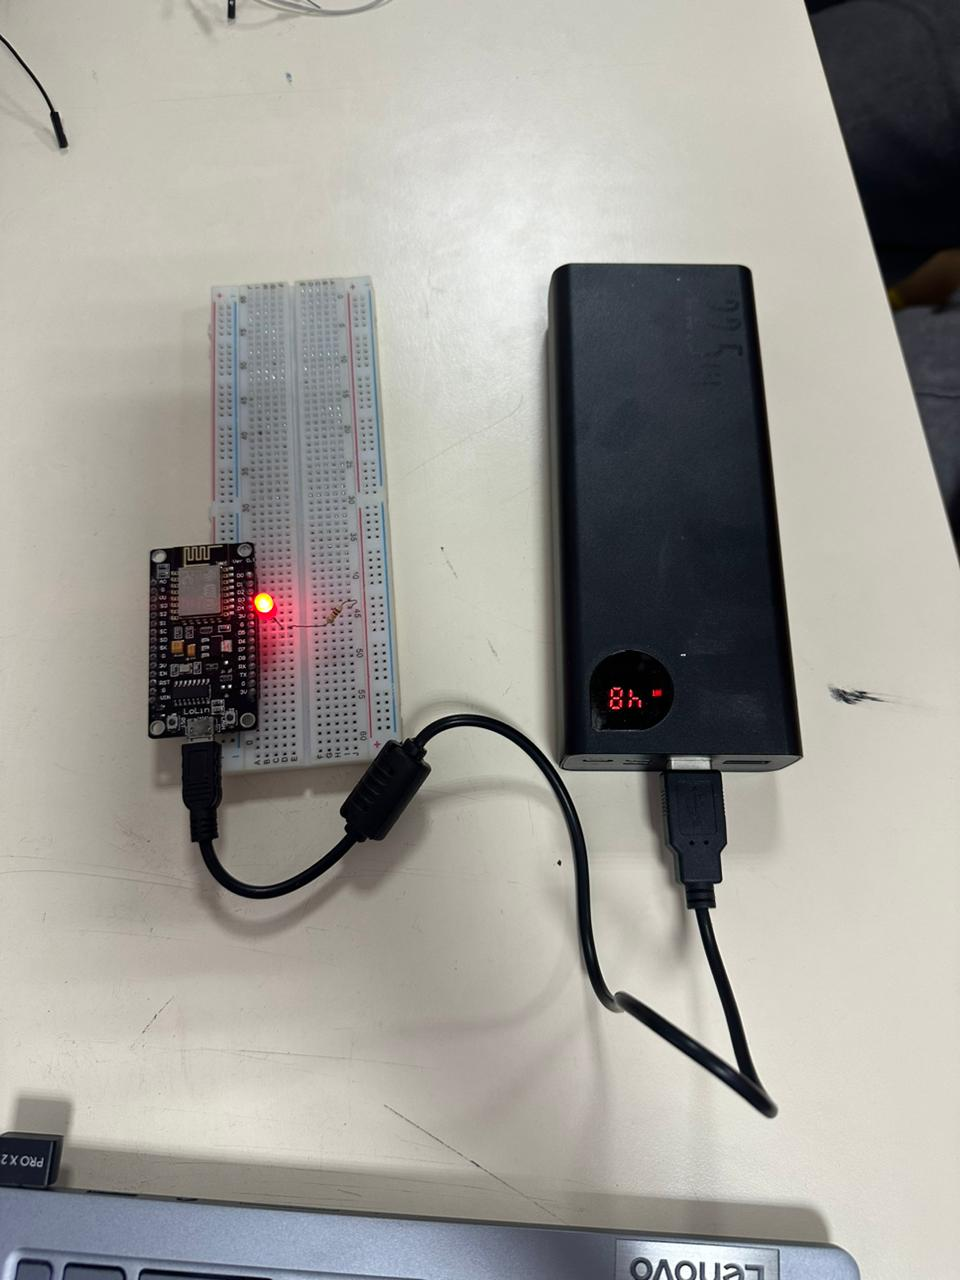
\includegraphics[width=0.6\textwidth]{../A15_Physical/circuit-on.jpeg}
    \caption{Circuit physique - LED allumée}
\end{figure}

\subsection*{Interface Node-RED}

\begin{figure}[H]
    \centering
    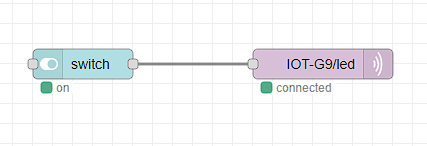
\includegraphics[width=0.7\textwidth]{../A15_Physical/flows.png}
    \caption{Flux Node-RED}
\end{figure}

\begin{figure}[H]
    \centering
    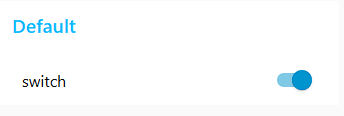
\includegraphics[width=0.7\textwidth]{../A15_Physical/dashboard.png}
    \caption{Dashboard Node-RED}
\end{figure}

\vspace{0.5cm}
\textbf{Code source :} Le code Arduino utilisé pour cet atelier est disponible sur notre dépôt GitHub à l'emplacement : \texttt{A15\_Physical/sketch/sketch.ino}.

\clearpage

\section*{Atelier 15 - Question 7 (Q07)}

\textbf{Description :} Réalisation physique d'un système qui lit le niveau d'eau via un capteur (pin \texttt{A0}) et le publie sur MQTT, tout en écoutant des commandes pour contrôler une LED. Les données sont envoyées et reçues via le NodeMCU.

\vspace{0.5cm}

\subsection*{Montage Circuit}

\begin{figure}[H]
    \centering
    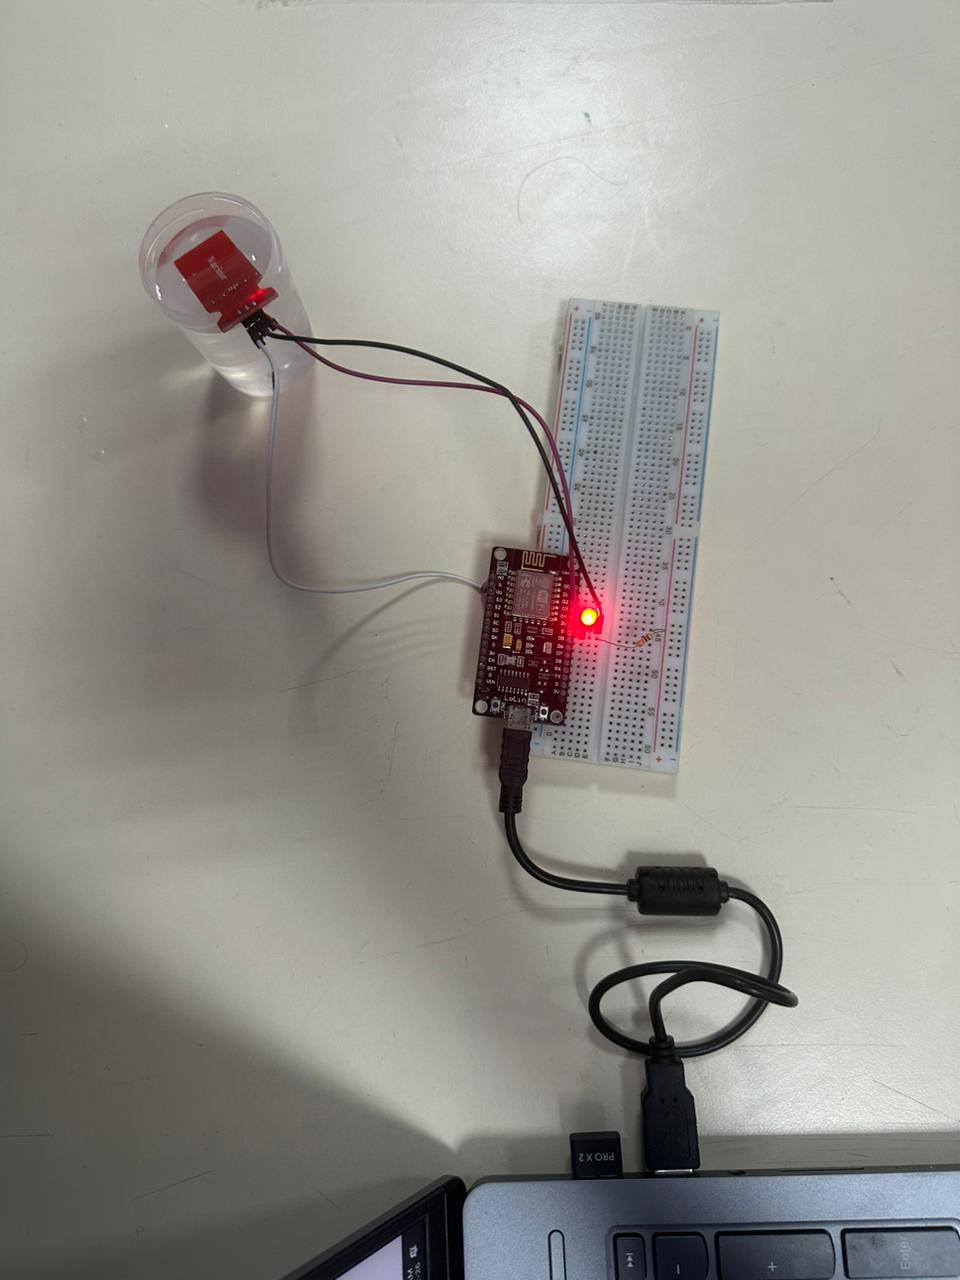
\includegraphics[width=0.6\textwidth]{../A15_Physical/Q07/circuit-1.jpeg}
    \caption{Circuit physique - Vue 1}
\end{figure}

\begin{figure}[H]
    \centering
    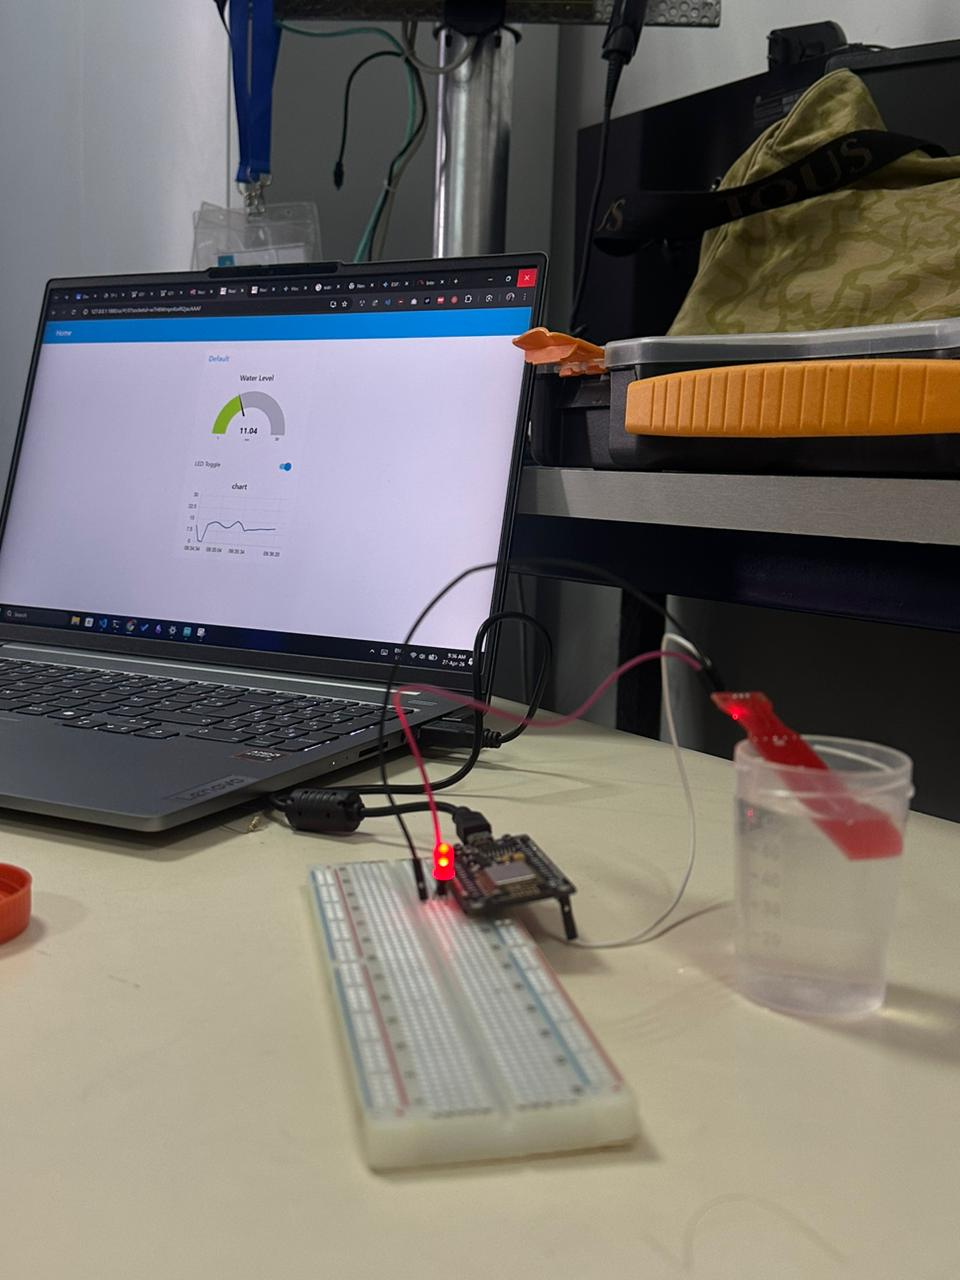
\includegraphics[width=0.6\textwidth]{../A15_Physical/Q07/circuit-2.jpeg}
    \caption{Circuit physique - Vue 2}
\end{figure}

\subsection*{Interface Node-RED}

\begin{figure}[H]
    \centering
    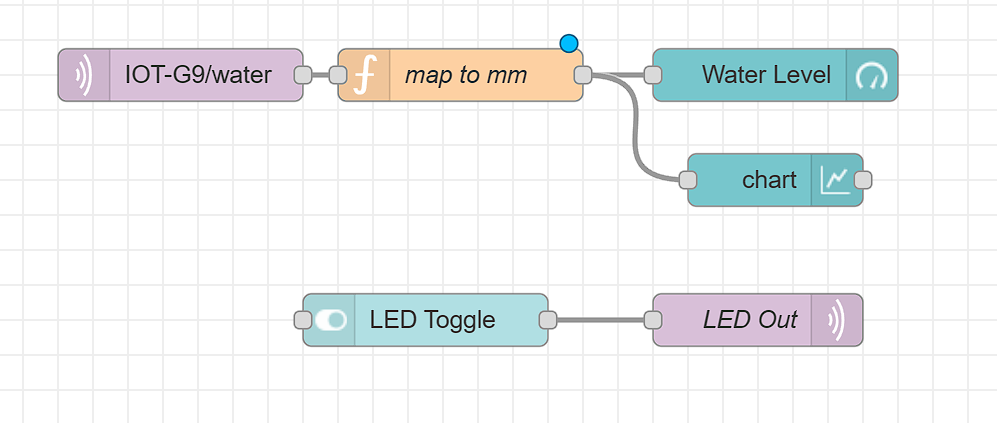
\includegraphics[width=0.7\textwidth]{../A15_Physical/Q07/flows.png}
    \caption{Flux Node-RED - Capteur d'eau et LED}
\end{figure}

\begin{figure}[H]
    \centering
    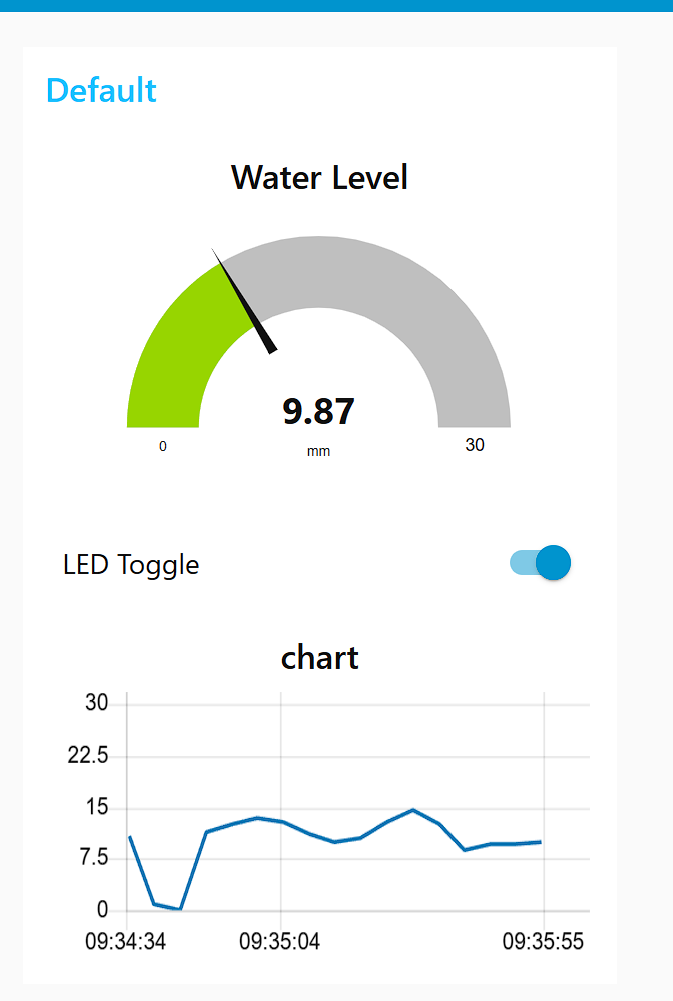
\includegraphics[width=0.7\textwidth]{../A15_Physical/Q07/dashboard.png}
    \caption{Dashboard Node-RED - Capteur d'eau et LED}
\end{figure}

\vspace{0.5cm}
\textbf{Code source :} Le code Arduino utilisé pour cette question est disponible sur le dépôt GitHub à l'emplacement : \texttt{A15\_Physical/Q07/sketch/sketch.ino}.

\clearpage

\section*{Atelier 15 - Question 8 (Q08)}

\textbf{Description :} Utilisation de MediaPipe pour détecter le pincement des doigts (hand finger pinch) afin de contrôler une LED. L'état du pincement (ouvert/fermé) est détecté par caméra et envoyé via MQTT pour allumer ou éteindre la LED sur le NodeMCU.

\vspace{0.5cm}

\subsection*{Fonctionnement de la détection (MediaPipe)}

Nous avons développé un script Python utilisant la bibliothèque \textbf{MediaPipe} de Google pour la détection et le suivi des points de repère (landmarks) de la main en temps réel via une webcam. Le script calcule la distance euclidienne entre le bout du pouce (landmark 4) et le bout de l'index (landmark 8). 

Si cette distance est inférieure à un seuil défini, le système considère qu'il y a un pincement (pinch) et publie le message \texttt{on} sur le broker MQTT pour allumer la LED. Lorsque les doigts s'écartent, il publie \texttt{off} pour l'éteindre.

\vspace{0.5cm}
\textbf{Code source :} Le script Python est disponible sur le dépôt GitHub à l'emplacement : \texttt{A15\_Physical/Q08/main.py}.

\subsection*{Montage Circuit}

\begin{figure}[H]
    \centering
    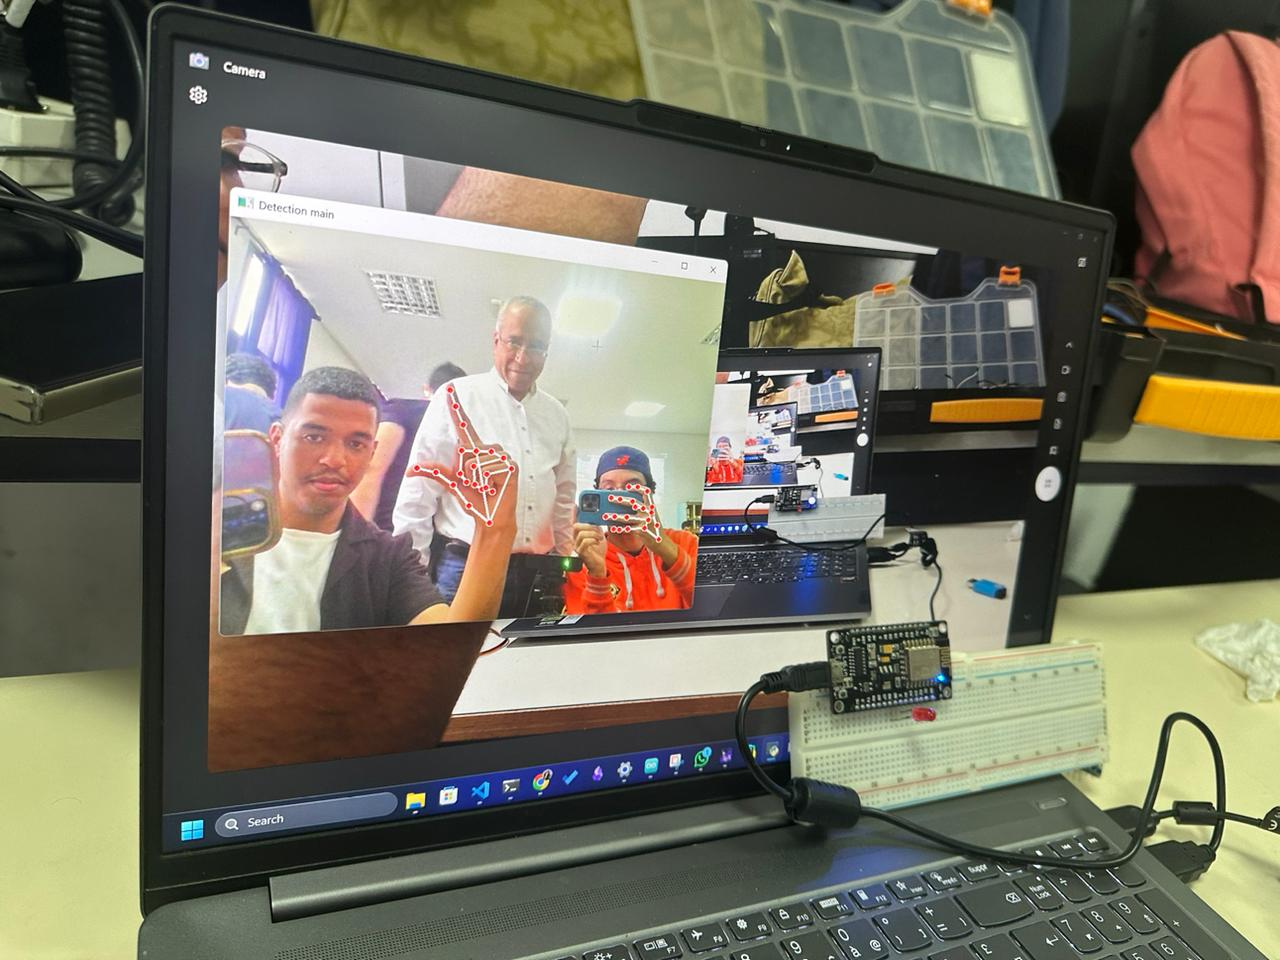
\includegraphics[width=0.6\textwidth]{../A15_Physical/Q08/circuit-pinch-off.jpeg}
    \caption{Circuit physique - LED éteinte (pas de pincement)}
\end{figure}

\begin{figure}[H]
    \centering
    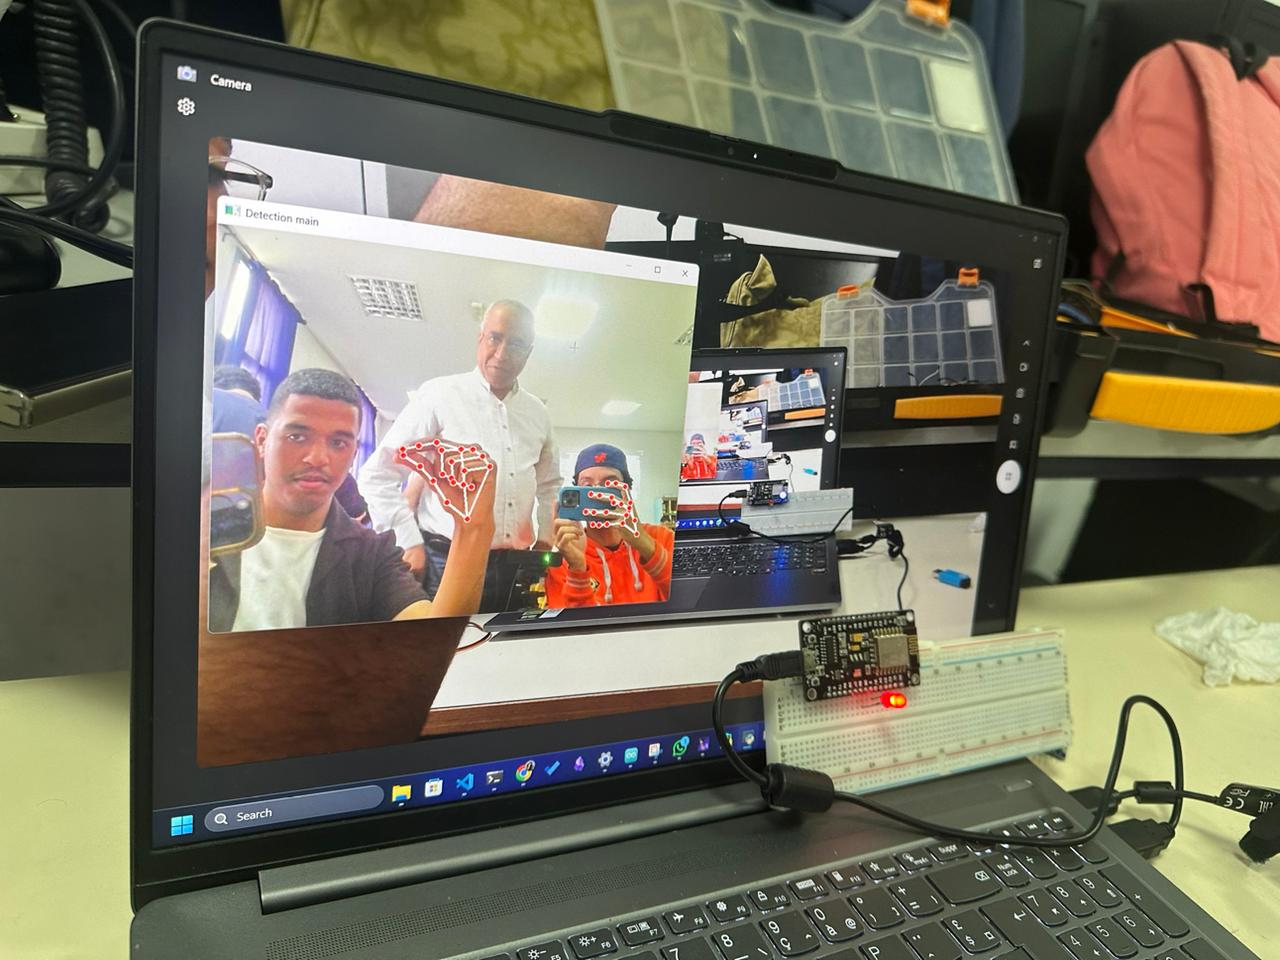
\includegraphics[width=0.6\textwidth]{../A15_Physical/Q08/circuit-pinch-on.jpeg}
    \caption{Circuit physique - LED allumée (pincement détecté)}
\end{figure}

\subsection*{Cas d'utilisation de MediaPipe dans l'IoT}

L'intégration de la reconnaissance gestuelle via MediaPipe avec les systèmes IoT offre des possibilités très intéressantes dans plusieurs domaines :
\begin{itemize}
    \item \textbf{Domotique sans contact :} Contrôler l'éclairage ou les appareils (ex: dans la cuisine) sans utiliser d'interrupteurs physiques lorsque les mains sont mouillées ou sales.
    \item \textbf{Milieu médical :} Permettre au personnel de santé de manipuler des interfaces ou des équipements médicaux à distance, réduisant ainsi le risque de contamination croisée.
    \item \textbf{Accessibilité :} Offrir une interface alternative pour les personnes à mobilité réduite, leur permettant de contrôler leur environnement via de simples gestes.
    \item \textbf{Sécurité industrielle :} Contrôler des machines dangereuses à distance, ou valider des commandes avec des gestes spécifiques.
\end{itemize}

\end{document}
